\subsection{Q3 - Sistema Operativo da VM Metasploitable 2}

Nesta secção ir-se-á descrever como foi detetado o Sistema Operativo da Metasploitable 2 através do NMap.Explicando sucintamente como o próprio Nmap o faz.Analisando também os resultados obtidos.

O comando utilizado para reconhecer o sistema operativo usado pela VM Metasploitable 2 foi:
\begin{lstlisting}
nmap -O 172.16.130
\end{lstlisting}

O comando faz a deteção do sistema operativo através de TCP/IP fingerprinting,isto é, envia pacotes TCP e UDP para examinar os bits que se encontram nas respostas.Alguns dos testes realizados são o tamanho inicial da janela, o suporte a certa opções do TCP entre outros.Seguidamente, compara com a base dados de fingerprint para tentar reconhecer o sistema operativo que daria essas respostas.

Atraves das funcionalidades do Zenmap foi extraido o resultado do scan para um xml que se encontra em Anexo \ref{sec:NmapOS}.Na resposta podemos ver também os serviços ativos nas várias portas como o MAC.Ao continuar a ler a resposta podemos ver que a maquina analisada corre um sistema operativo Linux entre as versões 2.6.9 e 2.6.33 com o kernel linux.kernel: 2.6.Na tag do XML \textless os\textgreater podemos quais as portas usadas e sobre que protocolo tal como a accuracy do resultado que , neste caso, é de 100\%.


\subsection{Q4 - Serviços Ativos na VM Metasploitable 2}

Nesta questão ir-se-á descrever como foram detetados os serviços ativos na maquina Metaexploitable 2 utilizando o Nmap e, como este o faz.Seguidamente dos serviços detetados analisar-se-á o CVE mais recente para três desses serviços,ou seja, o CVE mais recente para cada um dos serviços escolhidos.

Os serviços ativos do sistema VM Metasploitable 2 foram detados utilizando o comando :

\begin{lstlisting}

nmap -sV --version-all

\end{lstlisting}

O comando foi utilizado com a flag \"version-all\" de forma a receber o maior detalhe sobre os serviçoes e as suas versões.Contudo esta metodologia pode ser mais facilmente detetada.

O Nmap utiliza probes especializadas para detetar as versões dos serviços através das respostas que estes devolvem. Este tenta descobrir desde o protocolo usado , o serviço localizado na porta como a versão do mesmo , caso possível.

O resultado gerado por o nmap e extraido para um XML encontra-se no Anexo \ref{sec:NmapServices}
Através do resultado podemos concluir que existem 23 portas abertas.Nestas encontram-se varios serviços ativos entre eles um servidor Apache na versão 2.2.8 , um implementaçao do SSH (OpenSSH 4.7p1) e também uma base de dados PostgreSQL DB que se encontra entre as versões 8.3.0 e 8.3.7 . Realça-se a porta 6000 que apesar da porta estar aberta foi impossivel para o nmap descobrir a versão do serviço X11.Esta informação encontra se disponivel no texto do XML também como nas tags finais \textless port\textgreater onde se refere todos os campos que se refere no texto

Os serviços especificados anteriormente para as versões que se encontram instaladas sofrem das seguintes vulnerabilidades descritas nas seguintes seções.

\subsubsection{Apache 2.2.8}
\hfill\\

A vulnerabilidade mais recente encontrada afeta os servidores Apache 2.2.0 até 2.4.29.

Identificada por o CVE-2018-1312. A vulnerabilidade tem CVSS de 6.8 e um vetor de ataque descrito na figura seguinte.

\begin{figure}[h!]
	\centering
		
	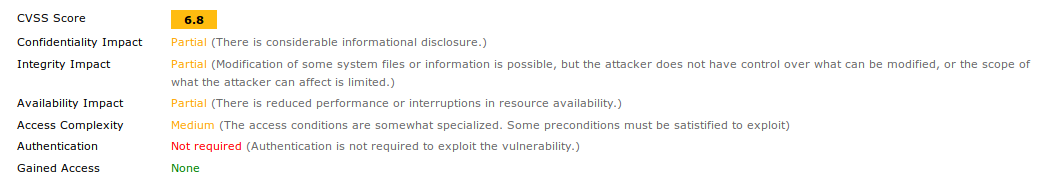
\includegraphics[width=\textwidth,height=3cm,keepaspectratio]{images/apacheCVE.png}
		
	\caption{Vetor de Ataque da CVE-2018-1312}
		
	\label{fig:apacheCVE}
\end{figure}

A vulnerabilidade torna o sistema a ataques por repetição visto que ao gerar o HTTP Digest authentification challenge o nonce utilizado para prever este tipo de ataques não é devidamente gerado utilizadando uma pseudo-random seed.Caso um Cluster de servers utilize a mesma configuração para o Digest, o atacante poderia repetir as HTTP requests para os vários servidores sem ser detetado.

\subsubsection{OpenSSH 4.7p1}
\hfill\\

A vulnerabilidade afeta todas as versões do OpenSSH antes da versao 7.5\_p1-r3 não inclusive.Identificada pelo CVE-2017-15906 tem CVSS de 5.0 e o seguinte vetor de ataque.


\begin{figure}[h!]
	\centering
		
	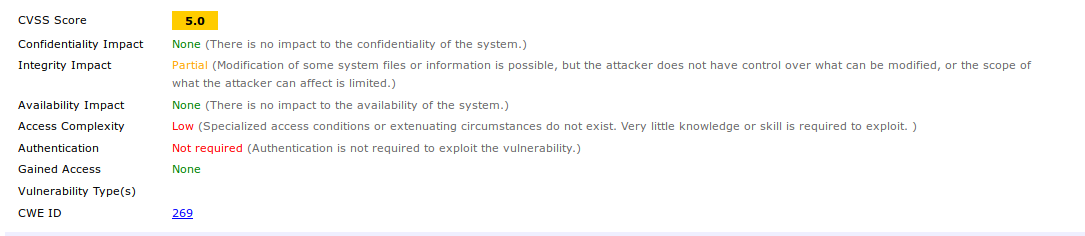
\includegraphics[width=\textwidth,height=3cm,keepaspectratio]{images/openSSHCVE.png}
		
	\caption{Vetor de Ataque do CVE-2017-15906}
		
	\label{fig:openSSH}
\end{figure}

A vulnerabilidade permite criar ficheiros com lenght zero por um atacante.Isto é possível visto que não é propriamente impedido ao atacante de utilizar operações de escrita no modo de readonly.Exatamente na função process\_open no ficheiro de código sftp-server.c.

\subsubsection{PostgreSQL 8.3.7}
\hfill\\

A versão do serviço não foi precisamente identificada.Por consequência, pesquisar-se-á por vulnerabilidades para a versão mais recente possível.

A vulnerabilidade afeta todas as versoes anteriores a 9 e quase todas antes da 10.5. Identificada pelo CVE-2018-1115 tem CVSS de 6.4 e o seu vetor de ataque esta descrito na figura seguinte.


\begin{figure}[h!]
	\centering
		
	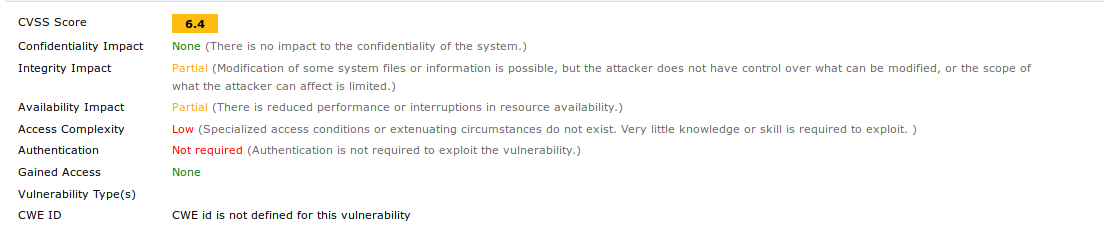
\includegraphics[width=\textwidth,height=3cm,keepaspectratio]{images/postgreSQLCVE.png}
		
	\caption{Vetor de Ataque do CVE-2018-1115}
		
	\label{fig:postgreSQL}
\end{figure}

A vulnerabilidade permite ,aos atacante que possam conetar-se a base de dados, em certos cenários, "crashar" o servidor ou distribuir as mensagens de log por ficheiros de log não desejados.É possível visto que o modulo "adminpack" instala uma função nova pg\_logfile\_rotate() que é um alias para uma função do próprio postgreSQL. Essa função built-in só deveria ser executada por superuser ,no entanto o alias pode ser executado por qualquer utilzador.

\clearpage